\documentclass[../../main.tex]{subfiles}

\begin{document}

\setchapterpreamble[u]{\margintoc}

\chapter{深度优先搜索和广度优先搜索}

深度优先搜索的本质是一种暴力搜索,我们从一个节点开始,不断地向下搜索,直到无法继续搜索为止。然后我们回溯到上一个节点,
继续搜索。通常这个回溯是通过递归的方式形成的,如果在搜索的过程中,我们需要记录搜索的节点,则我们需要伴随递归的自动
回溯对记录的数据进行删除和新增。

广度优先搜索的本质是一种暴力搜索,我们从一个节点开始,通过队列保存当前节点的所有子节点,然后不断地从队列中取出节点,
直到队列为空为止。

实际上,在树的章节中,我们已经使用过了很多次深度优先搜索和广度优先搜索的理念。

\section{组合问题}

组合问题是深度优先搜索结合回溯并去重的典型应用。我们可以通过画出递归树来分析组合问题,其本质也是我们解决许多
问题的思路。

\subsection{\href{https://leetcode.cn/problems/combinations/}{组合}}
\label{subsec:combinations}

我们需要实现一个$1..n$的组合。同样地画出123组合两个数的递归树。同时我们可以实现一定的剪枝操作。

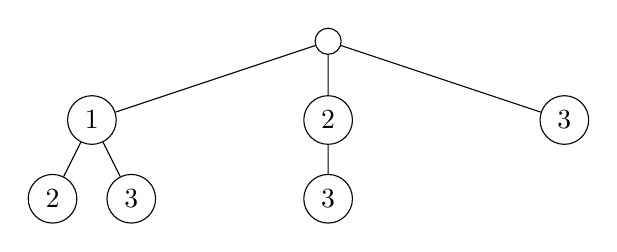
\begin{tikzpicture}[level distance=1cm,
  level 1/.style={sibling distance=3cm},
  level 2/.style={sibling distance=1cm}]
  \node[circle,draw] { }
    child {
      node[circle,draw] {1}
      child {
        node[circle,draw] {2}
      }
      child {
        node[circle,draw] {3}
      }
    }
    child {
      node[circle,draw] {2}
      child {
        node[circle,draw] {3}
      }
    }
    child {
      node[circle,draw] {3}
    };
\end{tikzpicture}

\lstinputlisting[language=C++]{code/combinations.cpp}

\subsection{\href{https://leetcode.cn/problems/combination-sum/}{组合总和}}
\label{subsec:combination-sum}

这个题与\ref{subsec:combinations}类似,由于没有重复的数字,所以我们不需要进行去重操作。由于可以重复使用元素,
所以我们需要重新画出递归树,如下图所示。以数组$[1, 2, 3]$为例。对于值为1的节点,其选择的元素为$[1, 2, 3]$,
对于值为2的节点,其选择的元素为$[2, 3]$,对于值为3的节点,其选择的元素为$[3]$。

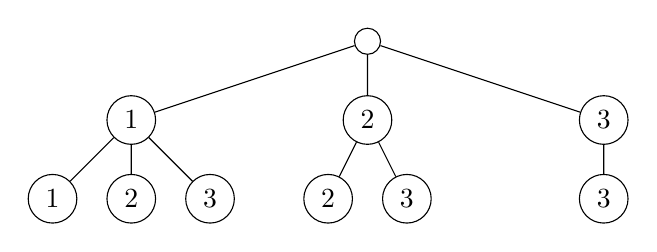
\begin{tikzpicture}[level distance=1cm,
  level 1/.style={sibling distance=3cm},
  level 2/.style={sibling distance=1cm}]
  \node[circle,draw] { }
    child {
      node[circle,draw] {1}
      child {
        node[circle, draw] {1}
      }
      child {
        node[circle,draw] {2}
      }
      child {
        node[circle,draw] {3}
      }
    }
    child {
      node[circle,draw] {2}
      child {
        node[circle,draw] {2}
      }
      child {
        node[circle,draw] {3}
      }
    }
    child {
      node[circle,draw] {3}
      child {
        node[circle,draw] {3}
      }
    };
\end{tikzpicture}

通过上述的分析,我们可以得出如下的代码:

\lstinputlisting[language=C++]{code/combination-sum.cpp}

\begin{kaobox}[title=类似题目]
  解决了这个题目,你就可以非常容易地解决\href{https://leetcode.cn/problems/combination-sum-iii/}
  {组合总和 III}了。
\end{kaobox}

\subsection{\href{https://leetcode-cn.com/problems/combination-sum-ii/}{组合总和 II}}

本题与\ref{subsec:combination-sum}看似类似,实际上有很大的差别。该题最大的差别就在于去重。
我们仍然需要通过画出递归树来分析,例如元素为$[3,3,2,2,1,1]$。我们可以发现,对于值为3的节点,
其选择的元素为$[3, 2, 1]$,对于值为2的节点,其选择的元素为$[2, 1]$,对于值为1的节点,其选择的元素为$[1]$。
显然,本质就是我们需要在每一层实现去重,每一次都不能访问到相同的元素。

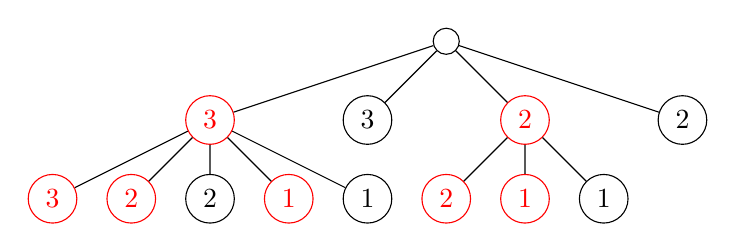
\begin{tikzpicture}[level distance=1cm,
  level 1/.style={sibling distance=2cm},
  level 2/.style={sibling distance=1cm}]
  \node[circle,draw] { }
    child {
      node[circle,draw, color=red] {3}
      child {
        node[circle, draw, color=red] {3}
      }
      child {
        node[circle,draw, color=red] {2}
      }
      child {
        node[circle,draw] {2}
      }
      child {
        node[circle,draw, color=red] {1}
      }
      child {
        node[circle,draw] {1}
      }
    }
    child {
      node[circle,draw] {3}
    }
    child {
      node[circle,draw,color=red] {2}
      child {
        node[circle,draw, color=red] {2}
      }
      child {
        node[circle,draw, color=red] {1}
      }
      child {
        node[circle,draw] {1}
      }
    }
    child {
      node[circle,draw] {2}
    };
\end{tikzpicture}

显然,要实现同层去重,我们有两种方式:

\begin{itemize}
  \item 在每一层构建一个哈希表,用于记录当前层已经访问过的元素。
  \item 对数组进行排序,然后在每一层,如果当前元素与上一个元素相同,则跳过。
\end{itemize}

\lstinputlisting[language=C++]{code/combination-sum-ii.cpp}

\section{分割问题}

分割问题是深度优先搜索结合回溯的典型应用。我们可以通过画出递归树来分析分割问题\sidenote{去思考递归树
永远是解决该类问题的首要思考手段}。

\subsection{\href{https://leetcode.cn/problems/palindrome-partitioning/}{分割回文串}}

我们可以通过画出递归树来分析分割回文串问题。例如,对于字符串\texttt{"aab"},我们可以得到如下的递归树:

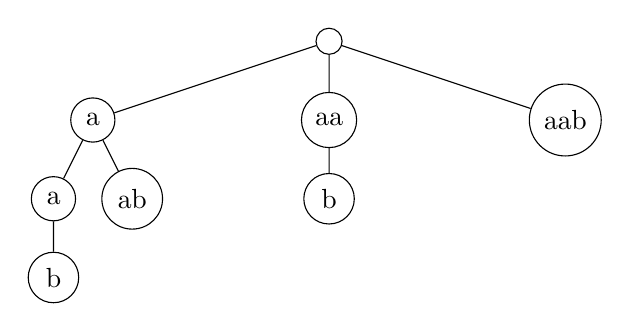
\begin{tikzpicture}[level distance=1cm,
  level 1/.style={sibling distance=3cm},
  level 2/.style={sibling distance=1cm}]
  \node[circle,draw] { }
    child {
      node[circle,draw] {a}
      child {
        node[circle,draw] {a}
        child {
          node[circle,draw] {b}
        }
      }
      child {
        node[circle,draw] {ab}
      }
    }
    child {
      node[circle,draw] {aa}
      child {
        node[circle,draw] {b}
      }
    }
    child {
      node[circle, draw] {aab}
    };
\end{tikzpicture}

从上述的递归树,我们可以非常容易的得到思路。首先每一层我们的操作都是类似的,都是从当前递归树的深度到
字符串的长度进行切割,然后判断切割的字符串是否是回文串。其终止的条件就是处理完了整个字符串。于是
我们可以得到如下代码:

\lstinputlisting[language=C++]{code/palindrome-partitioning.cpp}

\subsection{\href{https://leetcode.cn/problems/restore-ip-addresses/}{复原IP地址}}

这个问题本质仍然是分割,其解决的思路与上题是一致的。唯一的不同就在于我们分割的数目,在这个题中我们分割
的数目为1-3。实际上,我给出的代码没有进行剪枝,所以效率会稍微低一些。

\lstinputlisting[language=C++]{code/restore-ip-addresses.cpp}

\section{子集问题}

\subsection{\href{https://leetcode-cn.com/problems/subsets/}{子集}}

这个题可以使用两种做法,首先介绍作为一个正常人类能够思考出来的方法:

\begin{itemize}
  \item $[]$: $[]$
  \item $[1]$ : $[], [1]$
  \item $[1, 2]$ : $[], [1], [2], [1, 2]$
  \item $[1, 2, 3]$ : $[], [1], [2], [3], [1, 2], [1, 3], [2, 3], [1, 2, 3]$
\end{itemize}

假设$[a_{1}, a_{2}, \dots, a_{n}]$的子集为$\alpha$,则$[a_{1}, a_{2}, \dots, a_{n}, a_{n+1}]$的子集为

$$
\alpha \cup \{ \alpha_{i} \cup a_{n+1} \mid \alpha_{i} \in \alpha \}
$$

然后我们就很能容易地写出如下的代码:

\lstinputlisting[language=C++]{code/subsets-math.cpp}

我们仍然可以通过画出递归树解决子集问题。例如,对于数组$[1, 2, 3]$,我们可以得到如下的递归树。可以发现
如果我们沿着树搜索,每次我们到了一个新的节点,我们就能发现一个新的子集\sidenote{这个方法在我看来并不是
初学的人能够思考到的方法。反而上面的数学证明方法才是作为一个正常人的思维方式。}。:

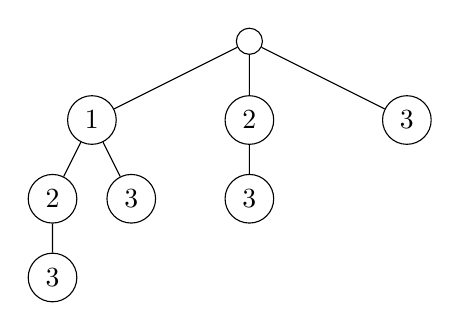
\begin{tikzpicture}[level distance=1cm,
  level 1/.style={sibling distance=2cm},
  level 2/.style={sibling distance=1cm}]
  \node[circle,draw] { }
    child {
      node[circle,draw] {1}
      child {
        node[circle,draw] {2}
        child {
          node[circle,draw] {3}
        }
      }
      child {
        node[circle,draw] {3}
      }
    }
    child {
      node[circle,draw] {2}
      child {
        node[circle,draw] {3}
      }
    }
    child {
      node[circle,draw] {3}
    };
\end{tikzpicture}

\lstinputlisting[language=C++]{code/subsets.cpp}

\subsection{\href{https://leetcode.cn/problems/subsets-ii/}{子集 II}}

这次我们的任务需要去重了。我们仍然按照上面的思维方式,从两个角度出发去重,首先是从数学的角度去重,例如
数组$[a_{1}, a_{2}, a_{3}, \dots ,a_{n - 1}, a_{n}]$。我们设数组$a_{1}, a_{2}, a_{3}, \dots ,a_{n - 1}$
的子集为$\alpha$。设数组$[a_{1}, a_{2}, a_{3}, \dots ,a_{n - 1}, a_{n}]$的子集为$\beta$。
我们可以轻易地得知$\beta = \sigma + \alpha$。当我们遇到了一个新的与$a_{n}$相同的元素$a_{n + 1}$
时,我们必须忽略到$\alpha$部分,不然我们就会得到一个新的$\beta$。所以,我们只对$\sigma$部分进行处理
即可\sidenote{
这样讲过于抽象了,为了方便理解举一个例子$[1,2,2]$。对于数组$[1]$来说其子集为$[], [1]$。数组$[1,2]$
的子集为$[], [1] ,[2], [1, 2]$。当再添加一个$[2]$,我们不能再处理$[], [1]$了,因为我们已经在最初的
$2$中进行过操作了。所以我们只需要处理$[2], [1, 2]$,变为$[], [1], [2], [1, 2], [2, 2], [1, 2, 2]$。
同样地,如果再添加一个$2$,我们只需要处理$[2, 2], [1, 2, 2]$。
}。

因此,我们可以先对数组进行排序,然后按照这个思路实现处理。

\lstinputlisting[language=C++]{code/subsets-ii-math.cpp}

同样地我们也可以基于递归树的方式实现去重。实际上,经过我们上面的分析,你已经能够很快地得出答案了。我们仍然
画出递归树,如同组合问题一样,对于同一层的元素相同值,我们必须忽略,所以仍然对数组进行排序。

\lstinputlisting[language=C++]{code/subsets-ii.cpp}

\begin{kaobox}[title=类似题目]
  在上面的题目中,我们是基于排序的方式去重的,然而如果不允许我们排序了,我们该如何处理了,很显然不在
  同层访问同一个元素,我们只需要使用一个哈希表记录就可以处理了。这样我们就可以处理
  \href{https://leetcode.cn/problems/non-decreasing-subsequences/}{递增子序列}
\end{kaobox}

\section{排列}

\subsection{\href{https://leetcode.cn/problems/permutations/}{全排列}}

我们画出全排列的递归树,以$123$的全排列为例,如下图所示。

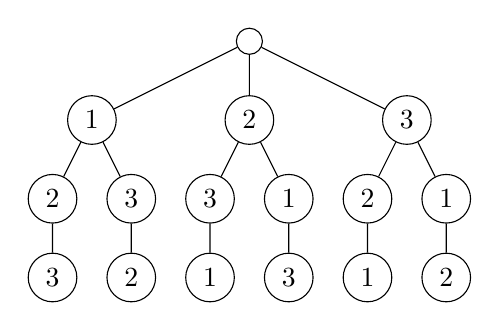
\begin{tikzpicture}[level distance=1cm,
  level 1/.style={sibling distance=2cm},
  level 2/.style={sibling distance=1cm}]
  \node[circle,draw] { }
    child {
      node[circle,draw] {1}
      child {
        node[circle,draw] {2}
        child {
          node[circle,draw] {3}
        }
      }
      child {
        node[circle,draw] {3}
        child {
          node[circle, draw] {2}
        }
      }
    }
    child {
      node[circle,draw] {2}
      child {
        node[circle,draw] {3}
        child {
          node[circle, draw] {1}
        }
      }
      child {
        node[circle,draw] {1}
        child {
          node[circle, draw] {3}
        }
      }
    }
    child {
      node[circle,draw] {3}
      child {
        node[circle,draw] {2}
        child {
          node[circle, draw] {1}
        }
      }
      child {
        node[circle,draw] {1}
        child {
          node[circle, draw] {2}
        }
      }
    };
\end{tikzpicture}

可见我们需要对所有的元素进行操作,只不过对于已经选择了的元素,我们不能再选择了。所以设置一个位图即可,这个位图
的状态随着递归的深度而改变。我们可以得到如下的代码:

\lstinputlisting[language=C++]{code/permutations.cpp}

\subsection{\href{https://leetcode.cn/problems/permutations-ii/}{全排列 II}}

同样的去重,其和组合没有本质的区别。不允许同层出现相同的元素,故排序后去重。

\lstinputlisting[language=C++]{code/permutations-ii.cpp}

\section{带有回溯的简单的深度优先搜索}

\subsection{\href{https://leetcode.cn/problems/letter-combinations-of-a-phone-number/}{电话号码的字母组合}}

要解决这个问题,我们仍然需要把递归树画出来,如下图所示,我们列举出了数字2和3的所有的组合。我们可以发现,我们
需要维护一个字符串,然后不断地向下搜索,直到字符串的长度等于输入的字符串的长度。然后我们回溯到上一个节点,继续搜索。
同时,我们需要维持一个变量,记录当前的搜索的位置,用于修改当前字符串的值。

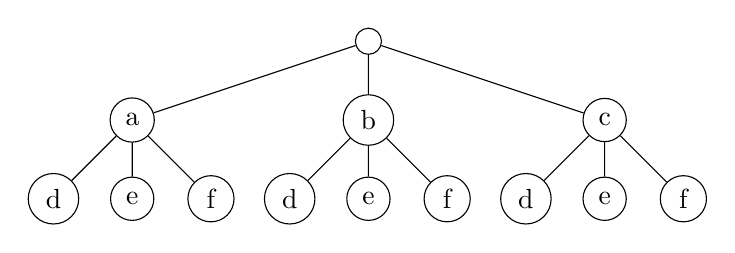
\begin{tikzpicture}[level distance=1cm,
  level 1/.style={sibling distance=3cm},
  level 2/.style={sibling distance=1cm}]
  \node[circle,draw] { }
    child {
      node[circle,draw] {a}
      child {
        node[circle,draw] {d}
      }
      child {
        node[circle,draw] {e}
      }
      child {
        node[circle,draw] {f}
      }
    }
    child {
      node[circle,draw] {b}
      child {
        node[circle,draw] {d}
      }
      child {
        node[circle,draw] {e}
      }
      child {
        node[circle,draw] {f}
      }
    }
    child {
      node[circle,draw] {c}
      child {
        node[circle,draw] {d}
      }
      child {
        node[circle,draw] {e}
      }
      child {
        node[circle,draw] {f}
      }
    };
\end{tikzpicture}

\lstinputlisting[language=C++]{code/letter-combinations-of-a-phone-number.cpp}

\subsection{\href{https://leetcode.cn/problems/generate-parentheses/}{括号生成}}

首先我们需要明确对于数字$n$总共有多少个左括号和右括号,我们可以发现,左括号的个数和右括号的个数都是$n$个。
同时,我们必须明确有效的含义:

\begin{itemize}
  \item 对于左括号而言,我们不需要做任何的检测,因为我们可以无限制的加入左括号直到$n$个。
  \item 对于右括号而言,当且仅当其数目小于左括号的数目时,我们才能够加入右括号。
\end{itemize}

我们可以使用深度优先搜索的思想,不断地向下搜索,直到左括号和右括号的数目都为$n$为止。我们需要维护一个字符串,
其大小为$2n$,然后不断地向下搜索,直到字符串的长度等于$2n$。然后我们回溯到上一个节点,继续搜索。同时,我们需要
维持两个变量,分别记录左括号和右括号的数目。

\lstinputlisting[language=C++]{code/generate-parentheses.cpp}

\end{document}
